\documentclass[12pt,a4paper,onecolumn]{article}
\usepackage[utf8]{inputenc}
\usepackage[english]{babel}
\usepackage{microtype}
\usepackage[style=apa,backend=biber]{biblatex}
\addbibresource{references.bib}
\usepackage{lscape}
\usepackage{csquotes}
\usepackage{graphicx}
\graphicspath{ {./images/} }
\usepackage{setspace}
\usepackage{upgreek}
\usepackage{authblk}
\usepackage{array}
\usepackage{color}
\usepackage{ragged2e}
\usepackage{caption}
\usepackage{booktabs}
\captionsetup[table]{justification=centering, singlelinecheck=off}
\usepackage{multirow}
\usepackage[breaklinks]{hyperref}
\usepackage{flafter}
\usepackage{float}
\usepackage{footnote}
\usepackage{afterpage}
\usepackage{subcaption}
\usepackage{listings}
\usepackage[margin=1.0in]{geometry}
\usepackage{amsmath}
\usepackage{amssymb}
\usepackage{siunitx}
\usepackage{dcolumn}
\usepackage[section]{placeins}
\usepackage{titlesec}
\usepackage{array}
\usepackage{abstract}
\usepackage{fancyhdr}

% NBER-style title and author formatting
\usepackage{authblk}
\renewcommand\Authfont{\fontsize{14}{16.8}\selectfont}
\renewcommand\Affilfont{\fontsize{12}{14.4}\selectfont}

% Reduce font size for table content to 9 pt
\let\oldtabular\tabular
\let\endoldtabular\endtabular
\renewenvironment{tabular}{\small\oldtabular}{\endoldtabular}

% Minimize white space between columns
\setlength{\tabcolsep}{4pt}

% Align numbers to the right, text to the left
\newcolumntype{L}[1]{>{\raggedright\let\newline\\\arraybackslash\hspace{0pt}}m{#1}}
\newcolumntype{C}[1]{>{\centering\let\newline\\\arraybackslash\hspace{0pt}}m{#1}}
\newcolumntype{R}[1]{>{\raggedleft\let\newline\\\arraybackslash\hspace{0pt}}m{#1}}

% NBER-style section headings
\titleformat{\section}
  {\normalfont\Large\bfseries}{\Roman{section}.}{1em}{}
\titleformat{\subsection}
  {\normalfont\large\bfseries}{\Alph{subsection}.}{1em}{}
\titleformat{\subsubsection}
  {\normalfont\normalsize\bfseries}{\arabic{subsubsection}.}{1em}{}

% Center and number equations
\numberwithin{equation}{section}

% Use a consistent font and size for all mathematical notation
\usepackage{mathptmx}

% NBER-style abstract
\renewcommand{\abstractnamefont}{\normalfont\large\bfseries}
\renewcommand{\abstracttextfont}{\normalfont\small}
\setlength{\absleftindent}{0.1\textwidth}
\setlength{\absrightindent}{0.1\textwidth}

% R code listing style
\lstset{ 
  language=R,  
  basicstyle=\small\ttfamily,
  numbers=left,               
  numberstyle=\tiny\color{gray}, 
  stepnumber=1,                  
  numbersep=5pt,                 
  backgroundcolor=\color{white},  
  showspaces=false,        
  showstringspaces=false,   
  showtabs=false,
  frame=single, 
  rulecolor=\color{black}, 
  tabsize=2, 
  captionpos=b,   
  breaklines=true,
  breakatwhitespace=false,
  keywordstyle=\color{blue}, 
  commentstyle=\color{green},
  stringstyle=\color{red}
}

% NBER-style header and footer
\pagestyle{fancy}
\fancyhf{}
\renewcommand{\headrulewidth}{0pt}
\fancyfoot[C]{\thepage}

% Title and author
\title{\vspace{-2cm}\Large\textbf{Oaxaca-Blinder decomposition}}
\author[]{Beatriz Gietner\thanks{Email: b.gietner@gmail.com}}
\affil{University College Dublin}
\date{}
\title{Oaxaca Paper}
\author{Beatriz Salvan Gietner Behr}
\date{August 2024}

\begin{document}

\maketitle

\section{Possible research questions}

a) How do cognitive and noncognitive skills differentially contribute to the gender achievement gap in Maths and English?

b) To what extent can socioeconomic factors and school characteristics explain the observed gender differences in academic performance?

c) How does the composition of the gender achievement gap vary across different levels of household income and parental education?

d) What role do specific noncognitive skills (e.g., Conscientiousness, Focused behaviour) play in widening or narrowing the gender achievement gap?

e) How do the unexplained portions of the gap differ between Maths and English, and what might this suggest about gender-specific returns to skills or potential discrimination?

Variables to consider: 

a) School characteristics: single-sex vs. mixed schools, proportion of male/female teachers in the school. \textcite{lee2018}

b) Teacher characteristics: teacher gender (especially for math and science subjects), teacher's gender biases or stereotypes (if measured).  \textcite{dee2007}

c) Parental expectations and attitudes: differential expectations for boys and girls, parental attitudes towards gender roles in education and careers. \textcite{jacobs2002} 

d) Peer effects: gender composition of peer groups
Prevalence of gender stereotypes among peers

e) Subject-specific self-efficacy: self-efficacy in math and science for girls, self-efficacy in reading and writing for boys.

f) Stereotype threat: awareness of gender stereotypes in academic domains, experiences of stereotype threat in test-taking situations.

g) Extracurricular activities: participation in gender-typed activities (e.g., sports, drama, STEM clubs).

h) Career aspirations: gender-typicality of career aspirations, perceived barriers to certain career paths based on gender.

i) Role models: exposure to same-gender role models in various academic fields.

k) Gender identity and expression: strength of gender identification, adherence to traditional gender norms.

l) Media and technology use: exposure to gendered media content, patterns of technology use that may differ by gender. 

m) Time use: time spent on household chores (often gendered), time allocation to different subjects or activities.

n) Subject choice: selection of elective subjects (if applicable at this age), intentions for future subject choices (e.g., for secondary school).

o) Parental involvement: differential patterns of mother's vs. father's involvement in schoolwork

p) Mental health and well-being: gender differences in anxiety, depression, or stress related to academics

q) Physical development: onset of puberty and its effects on academic performance (can differ by gender).

Ensure a strong theoretical basis for including each variable, citing relevant literature that demonstrates its differential impact on boys and girls.

Consider interaction effects between gender and these variables, as some factors may have different magnitudes of effect for boys versus girls.

Be cautious about potential endogeneity issues, especially with variables like subject choice or self-efficacy, which may be both causes and consequences of academic performance.

If possible, utilize longitudinal aspects of the Growing Up in Ireland data to examine how these factors' influences change over time.

Consider conducting separate decompositions for different subject areas (e.g., math, English, science) as the factors contributing to gender gaps often vary by domain.

School environment \textcite{legewie2014}

Gender stereotypes \textcite{cvencek2011,bian2017} 

Stereotype threat \textcite{spencer1999} 

Career aspirations \textcite{eccles1994,frome2006} 

Women in STEM \textcite{sax2008} 

Competitiveness \textcite{niederle2010} 

Cultural influences \textcite{guiso2008} 

Teacher anxiety effects \textcite{beilock2010} 

Gender similarities hypothesis \textcite{hyde2008} 

Effects of school type on stereotypes \textcite{blakemore2003} 

\section{Literature reviews}

The Oaxaca-Blinder decomposition, originally developed by \textcite{blinder1973} and  \parencite{oaxaca1973}, has become a widely used method in economics and social sciences for analyzing group differences in outcomes. In recent years, this technique has been increasingly applied to educational contexts to understand and decompose achievement gaps, particularly those related to gender. This section reviews recent studies that have employed the Oaxaca-Blinder decomposition to examine educational disparities.

\subsection{Gender Achievement Gaps}

Several recent studies have focused on decomposing gender achievement gaps in various educational settings. For instance, \parencite{golsteyn2014} applied the Oaxaca-Blinder decomposition to analyze gender differences in PISA test scores across multiple countries. They found that gender gaps in math, reading, and science could be partially explained by differences in noncognitive skills, particularly students' level of conscientiousness and test motivation.

Similarly, \parencite{gevrek2014} used this method to examine the gender gap in Maths performance in Turkey. Their results indicated that a significant portion of the gap could be attributed to differences in socioeconomic background and school characteristics, highlighting the importance of contextual factors in shaping educational outcomes.

\subsection{Cognitive and Noncognitive Skills}

The role of both cognitive and noncognitive skills in explaining achievement gaps has been a recurring theme in recent literature. \parencite{fortin2015} conducted a comprehensive study using Oaxaca-Blinder decomposition to analyze the gender gap in academic achievement across several countries. They found that noncognitive skills, particularly student attitudes and behaviors, played a crucial role in explaining the gap, often more so than cognitive abilities.

In a similar vein, \parencite{nguyen2020} applied the decomposition technique to examine gender differences in STEM (Science, Technology, Engineering, and Maths) achievement. The study revealed that while cognitive skills were important, noncognitive factors such as self-efficacy and interest in STEM subjects were key in explaining the persistent gender gap in these fields.

\subsection{Socioeconomic Factors and School Characteristics}

The impact of socioeconomic background and school characteristics on achievement gaps has also been a focus of recent research. \parencite{agasisti2021} used Oaxaca-Blinder decomposition to analyze the urban-rural achievement gap in Italy. Their findings suggested that differences in school resources and teacher quality were significant factors in explaining the gap, underscoring the importance of educational inputs.

Moreover, \parencite{cimpian2016} applied this method to investigate the gender gap in early reading achievement. They found that school-level factors, including classroom composition and teacher characteristics, played a substantial role in explaining the observed differences.

\subsection{Cross-Country Comparisons}

Several studies have utilized Oaxaca-Blinder decomposition for cross-country comparisons of educational gaps. \parencite{lounkaew2013} conducted a comparative analysis of the gender gap in educational attainment across Thailand and Vietnam. The study revealed that while family background was a significant factor in both countries, its impact varied considerably between the two, highlighting the importance of country-specific contexts.

Similarly, \parencite{karakolidis2016} used this technique to compare math and science achievement gaps across different European countries. Their results emphasized the varying roles of school systems and societal attitudes in shaping gender disparities in educational outcomes.

\section{Explaining the gender achievement-gap}

\begin{figure*}[ht] 
    \centering
    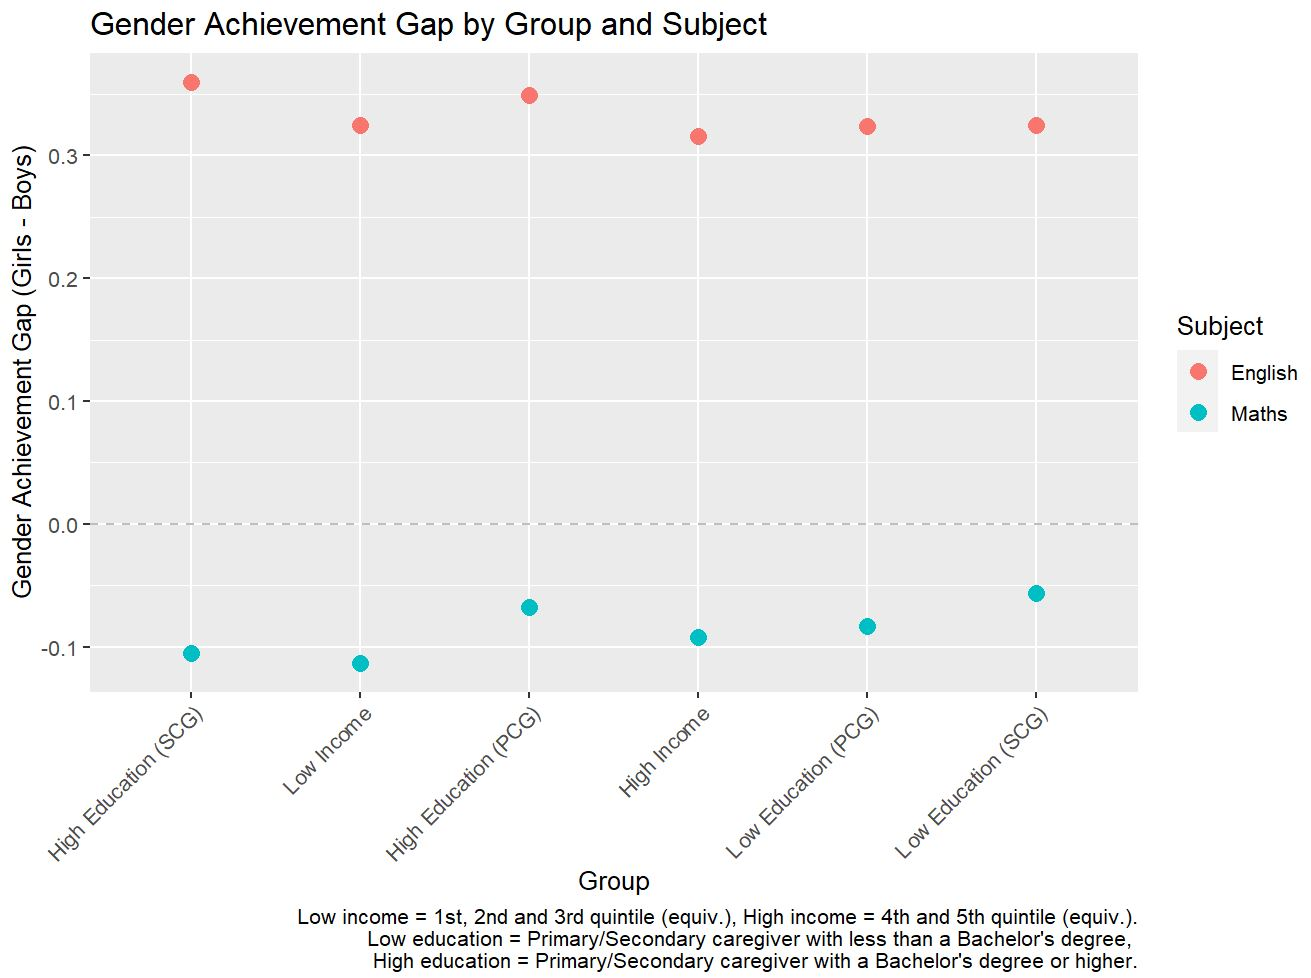
\includegraphics[width=1\linewidth]{Gender_gap_by_group.JPG}
    \caption{Gender Achievement Gap by Socioeconomic Group and Subject. This plot illustrates the gender achievement gap in English and Maths across different socioeconomic groups. The y-axis represents the gender gap, calculated as girls' mean score in the Junior Cert minus boys' mean score. Positive values indicate girls outperform boys, while negative values show boys outperform girls. The x-axis categories represent different income and parental education levels. Points above the dashed line ($y=0$) indicate a female advantage, while points below indicate a male advantage.}
    \label{fig:OBDecompGroup}
\end{figure*}

I began by creating two separate datasets, one for English scores and one for Maths scores. In each dataset, I included mean scores for girls and boys across different socioeconomic groups. These groups were based on household income levels (low income: 1st, 2nd, and 3rd quintiles; high income: 4th and 5th quintiles) and parental education levels (low education: less than a Bachelor's degree; high education: Bachelor's degree or higher). Next, I calculated the gender achievement gap for each group and subject. To do this, I subtracted the boys' mean score from the girls' mean score for each socioeconomic group in both English and Maths. Raw results are presented in Tables \ref{TableGenderAchievementGapMaths} and \ref{TableGenderAchievementGapEnglish}. This gave me a single value representing the gender gap, where a positive number meant girls outperformed boys, and a negative number meant boys outperformed girls. That is represented in Figure \ref{fig:OBDecompGroup}. Results show that across all income and education groups, boys outperform girls in Maths, and girls outperform boys in English. The achievement gap is also always smaller (in absolute values) in Maths than in English. 

For Maths, the gender achievement gap is largest in the low-income group and smallest in the primary caregiver high-education group (where the mother - for the majority of the sample - has at least a Bachelor's degree). Higher income and higher education levels, for both caregivers, are associated with better performance overall in Maths for both genders. The income effect (the difference in gender gaps - differences between boys' and girls' mean scores - between groups categorized by income level) is lower than the education effects (the difference, or gap, in means between groups - boys and girls - characterized by education levels of the caregivers), which suggests that parental education (especially of the secondary caregiver, which for the majority of the sample is the father) have a stronger influence in Maths performance than household income. Interestingly, household income and primary caregiver's education appear to narrow the achievement gap for Maths, while secondary caregiver's education widens it. Having a secondary caregiver with at least a bachelor's degree seem to have a positive effect on girls' Maths performance seeing that they are the group with the highest mean. The gender gap is wider in the high education secondary caregiver group compared to the low education secondary caregiver group, however, both girls and boys perform better in the high education secondary caregiver group, with girls showing a larger improvement compared to boys. This means that while the gender gap widens, girls still benefit from having a highly educated secondary caregiver, just not quite as much as boys do in terms of Maths performance. The gender ratios (the ratio between Girls Mean and Boys Mean) are all a bit below 1, which means that boys always perform better than girls across all groups in Maths, but the across-group difference is relatively small. The highest gender ratio in Maths is in the low education secondary caregiver group, meaning that the gender gap is smallest when the secondary caregiver has lower education levels. 

For English, the largest gender gap is observed in the group where the secondary caregiver has at least a Bachelor's degree, and the smallest in the high-income group. As with Maths, a higher household income is associated with better performance in English for both genders, and the gender gap decreases in higher income groups, which suggests that increased income can have a marginally stronger and positive effect on boys' performance. Higher education levels for both primary and secondary caregivers are associated with larger gender gaps, which indicates that girls might benefit more in English from having more educated caregivers.

For English, the gender ratios are all above 1, confirming girls' superior performance. The gender ratio is highest in the high education secondary caregiver group for English, mirroring the finding that this group also has the largest gender gap. This suggests that while higher secondary caregiver education benefits both genders in English, it appears to disproportionately benefit girls.

Overall, both income and caregiver education levels have a positive effect on Maths and English performances, and the effects of caregivers' education are stronger than the income effects, especially for Maths. 

The findings from this analysis have implications for our understanding of human capital formation and the economics of education. The persistent gender gaps in academic performance, particularly the male underperformance in English and female underperformance in Maths suggest potential inefficiencies in human capital accumulation. These gaps may lead to suboptimal educational and career choices, potentially affecting labor market outcomes and overall economic productivity \parencite{altonji1999race}.

The strong influence of cognitive factors on academic performance further emphasizes the importance of early skill formation, as championed by \textcite{heckman2006skill}. The differences in returns to cognitive and noncognitive skills between genders suggest that there might be gender-specific patterns in the production function of human capital, which could have implications for understanding wage differentials and occupational segregation later in the labor market \parencite{blau2017gender}.

Also the finding that socioeconomic and school-related factors mediate some of the gender differences in cognitive skills highlights the role of family background and educational inputs in shaping academic outcomes. This aligns with the literature on intergenerational transmission of human capital and the production function of cognitive and noncognitive skills \parencite{cunha2007technology}.

The varying gender gaps across different income and education levels suggest that the relationship between socioeconomic status and academic achievement is complex and potentially non-linear. This finding contributes to the ongoing debate about the relative importance of nature versus nurture in determining educational outcomes \parencite{sacerdote2011nature}.

The gender gaps in academic performance observed may have significant long-term economic consequences, particularly in terms of occupational segregation and wage differentials in the labor market. The underperformance of boys in English and girls in Maths could potentially lead to gender-based sorting into different educational tracks and, subsequently, into different occupations. This aligns with the theory of comparative advantage in occupational choice \parencite{rosen1978substitution}, where individuals select occupations based on their relative strengths.

As an example, the superior performance of girls in English might lead to their overrepresentation in humanities and social sciences, while boys' better performance in Maths could result in their dominance in STEM fields. This occupational segregation does have substantial implications for the labor market and the economy as a whole. \textcite{blau2017gender} argue that occupational segregation is a major contributor to the gender wage gap, as female-dominated occupations often pay less than male-dominated ones, even when controlling for skill levels and job characteristics.

Also, if these academic performance gaps persist into adulthood, they could contribute to skill differentials between men and women in the labor force. Given the increasing importance of both quantitative and communication skills in the modern economy \parencite{deming2017growing}, gender-based skill gaps would then lead to inefficient allocation of talent and reduced overall productivity.

My findings also relate to theories of statistical discrimination in labor markets \parencite{phelps1972statistical}. If employers believe that these gender differences in academic performance reflect underlying differences in skills or abilities, they might use gender as a proxy for productivity in hiring and promotion decisions. For example, an employer might be more inclined to hire a man for a maths-intensive job based on the average performance gap, even if the specific woman applicant is equally or more qualified, which then triggers a snowball effect, that could lead to a self-fulfilling prophecy where women, anticipating discrimination, invest less in maths skills, thus perpetuating the gap.

I have to note that these potential long-term consequences are speculative and based on the assumption that early academic performance gaps persist and translate into labor market outcomes. Longitudinal studies tracking individuals from school to the labor market would be necessary to confirm these hypotheses. 

\begin{table}[htbp]
\centering
\caption{Gender Achievement Gap in Maths by Socioeconomic Factors. This table presents mean Junior Certificate Maths scores for girls and boys across different income and parental education groups. Low-income levels are equivalent to the 1st, 2nd, and 3rd quintiles, while High-income accounts for the 4th and 5th quintiles. Parental education levels are separated by Low education (less than a Bachelor's degree) and High education (a Bachelor's degree or higher) for Primary caregiver (PCG) and Secondary Caregiver (SCG). It shows gender gaps (girls' mean minus boys' mean), overall mean scores, and gender ratios (girls' mean divided by boys' mean) for each group. Socioeconomic effects are calculated as the difference between high and low categories for each factor.}
\begin{tabular}{lccccc}
\hline
\multirow{2}{*}{Group} & \multicolumn{2}{c}{Mean Scores} & \multicolumn{3}{c}{Differences and Ratios} \\
\cmidrule(lr){2-3} \cmidrule(lr){4-6}
 & Girls Mean & Boys Mean & Gender Gap & Overall Mean & Gender Ratio \\
\hline
\multicolumn{6}{l}{\textbf{Group Data}} \\
Low Income & 9.235 & 9.348 & -0.113 & 9.292 & 0.988 \\
High Income & 10.075 & 10.167 & -0.092 & 10.121 & 0.991 \\
Low Education (PCG) & 9.371 & 9.454 & -0.083 & 9.413 & 0.991 \\
High Education (PCG) & 10.322 & 10.390 & -0.069 & 10.356 & 0.993 \\
Low Education (SCG) & 9.389 & 9.444 & -0.056 & 9.417 & 0.994 \\
High Education (SCG) & 10.333 & 10.438 & -0.105 & 10.386 & 0.990 \\
\hline
\multicolumn{6}{l}{\textbf{Socioeconomic Effects}} \\
Income Effect &  &  & 0.022 & 0.829 &  \\
PCG Education Effect &  &  & 0.014 & 0.943 &  \\
SCG Education Effect &  &  & -0.049 & 0.969 &  \\
\hline
\end{tabular}
\label{TableGenderAchievementGapMaths}
\end{table}

\begin{table}[htbp]
\centering
\caption{Gender Achievement Gap in English by Socioeconomic Factors. This table presents mean Junior Certificate English scores for girls and boys across different income and parental education groups. Low-income levels are equivalent to the 1st, 2nd, and 3rd quintiles, while High-income accounts for the 4th and 5th quintiles. Parental education levels are separated by Low education (less than a Bachelor's degree) and High education (a Bachelor's degree or higher) for Primary caregiver (PCG) and Secondary Caregiver (SCG). It shows gender gaps (girls' mean minus boys' mean), overall mean scores, and gender ratios (girls' mean divided by boys' mean) for each group. Socioeconomic effects are calculated as the difference between high and low categories for each factor.}
\begin{tabular}{lccccc}
\hline
\multirow{2}{*}{Group} & \multicolumn{2}{c}{Mean Scores} & \multicolumn{3}{c}{Differences and Ratios} \\
\cmidrule(lr){2-3} \cmidrule(lr){4-6}
 & Girls Mean & Boys Mean & Gender Gap & Overall Mean & Gender Ratio \\
\hline
\multicolumn{6}{l}{\textbf{Group Data}} \\
Low Income & 10.137 & 9.812 & 0.325 & 9.974 & 1.033 \\
High Income & 10.631 & 10.315 & 0.316 & 10.473 & 1.031 \\
Low Education (PCG) & 10.223 & 9.899 & 0.324 & 10.061 & 1.033 \\
High Education (PCG) & 10.764 & 10.414 & 0.349 & 10.589 & 1.034 \\
Low Education (SCG) & 10.223 & 9.898 & 0.325 & 10.060 & 1.033 \\
High Education (SCG) & 10.794 & 10.434 & 0.360 & 10.614 & 1.035 \\
\hline
\multicolumn{6}{l}{\textbf{Socioeconomic Effects}} \\
Income Effect &  &  & -0.009 & 0.499 &  \\
PCG Education Effect &  &  & 0.025 & 0.528 &  \\
SCG Education Effect &  &  & 0.035 & 0.553 &  \\
\hline
\end{tabular}
\label{TableGenderAchievementGapEnglish}
\end{table}

There are a few attempts to explain the observed patterns in gender achievement gaps across socioeconomic groups. Being in a higher-income household may contribute to narrowing the gap through some channels: higher incomes most likely result in increased access to educational resources, it might reduce stress due to economic stability, and also create the possibility of greater parental involvement in children's education \parencite{sirin2005}. For example, \textcite{davis2005} found that, on average, highly educated parents value education more highly, which then creates a more stimulating home environment while making them better equipped to assist with homework. The recurrent gender gaps across all levels point to the possibility of more or less ingrained societal expectations about gender roles in academic subjects. These gaps may also reflect differences in teaching methods, brain development patterns, or gender-specific interests and engagement levels \parencite{ceci2009}. Other interesting factors identified in the literature include stereotype threat, where awareness of negative stereotypes can impair performance \parencite{spencer1999}; differences in spatial skills development \parencite{levine2005}; and the influence of same-gender teachers as role models \parencite{beilock2010}. \textcite{huang2013} showed that gender differences in self-efficacy and academic self-concept, particularly in STEM fields, have also been shown to contribute to achievement gaps. In addition, cross-cultural studies suggest that societal gender equality is associated with reduced gender gaps in Maths achievement \parencite{guiso2008}. The relative absence of women in STEM fields may also perpetuate these gaps through a lack of visible role models \parencite{blickenstaff2005}. 

In terms of cognitive and noncognitive measures, boys score higher than girls, on average, in all cognitive measures in all waves, even when subsetting by parents' income and education levels. Girls only outperform boys in Junior Cert English scores. Boys also have higher means than girls in all control variables (SES status and school characteristics), even if there are fewer of them represented in the sample. Conversely, girls outperform boys in all noncognitive indicators except for Emotional Stability (Neuroticism) and Emotional Resilience. These results ask for a deeper analysis, so I employed the Oaxaca-Blinder decomposition \parencite{oaxaca1973,blinder1973}, or Kitagawa decomposition \parencite{kitagawa1955}, method to see from where exactly these differences in grades (girls score higher than boys in English, and boys score higher than girls in Maths) arise, if from the cognitive part of the model or the noncognitive one, and how much these differences matter to the final outcome (Junior Cert grades).

The Oaxaca-Blinder decomposition is a statistical method used to explain the differences in the means of an outcome variable between two groups. In my study, I used it to analyze the gender achievement gap in academic performance. This technique was independently developed by Ronald Oaxaca (1973) and Alan Blinder (1973), and has since become a standard tool in labour economics and other social sciences.  The decomposition divides the difference in outcomes between two groups into the "explained" and the "unexplained" part. The former portion of the difference is attributed to group differences in measurable characteristics or predictors (e.g., cognitive abilities, noncognitive skills), and the latter is the residual portion that cannot be accounted for by the observed characteristics. The "unexplained" part is often interpreted as a measure of discrimination or the effect of unobserved variables.

In the context of my study, the Oaxaca-Blinder decomposition allows me to quantify how much of the gender achievement gap in Maths and English could be attributed to differences in cognitive and noncognitive skills between boys and girls, and how much remained unexplained by these factors.
This method has been widely used in educational research. For example, \textcite{fortin2015} used it to decompose gender differences in academic achievement across several countries, while \textcite{niederle2010} applied this technique to analyze gender gaps in Maths performance.
The Oaxaca-Blinder decomposition has its flaws and caution in the interpretation of results is advised. As pointed out by \textcite{jones1984}, the choice of reference group can affect the results, and the unexplained portion should be carefully interpreted.

In the Oaxaca-Blinder decomposition, Female is Group 1 (= 0) and Male is Group 2 (= 1), so whenever we have a negative result in group differences (first panel of the tables), it means that the value from Group 2 is bigger than for Group 1, and the opposite holds. When we get a negative coefficient for the variables considered, it means that the variable is associated with mitigating or reducing the difference in outcomes between the two groups, in our case the variable contributes to reducing the gender achievement gap, and the opposite also holds (a positive coefficient contributes to increasing the gender achievement gap). The magnitude of the coefficients indicates how much they contribute to the size of the Endowments, Returns, and Interaction for the three-fold decomposition, and Explained and Unexplained parts of the two-fold decomposition. Both SDQ and TIPI as indicators of noncognition yield similar results when analyzing each subject (Maths and English). 

\begin{table*}[ht]
\centering
\caption{\textbf{Maths SDQ} Results - Threefold decomposition}
\label{Maths_OBD_SDQ_3F} 
\begin{tabular}{lcccr}
\toprule
& \multicolumn{4}{c}{\textbf{Maths Points}} \\
\cmidrule(lr){2-5}
& \textbf{I} & \textbf{II} & \textbf{III} & \textbf{IV} \\
\midrule
Female (Group 1) & 9.685*** & 9.685*** & 9.685*** & 9.685*** \\
Male (Group 2) & 9.803*** & 9.803*** & 9.803*** & 9.803*** \\
Difference & -0.118* & -0.118* & -0.118* & -0.118* \\
Endowments & -0.264*** & -0.255*** & -0.247*** & -0.244*** \\
Returns & 0.101* & 0.096* & 0.083 & 0.082 \\
Interaction & 0.045 & 0.041 & 0.046 & 0.044 \\
\midrule
\textbf{Endowments} & & & & \\
\midrule
Vocal reasoning & -0.071*** & -0.057*** & -0.064*** & -0.055*** \\
Numerical ability & -0.210*** & -0.192*** & -0.200*** & -0.187*** \\
Matrices & -0.014* & -0.014* & -0.015* & -0.015* \\
\hline
Emotional resilience & -0.019* & -0.016* & -0.017* & -0.015 \\
Good conduct & 0.001 & 0.001 & 0.001 & 0.001 \\
Focused behaviour & 0.049*** & 0.050*** & 0.051*** & 0.051*** \\
Positive peer relationships & 0.001 & 0.000 & 0.000 & 0.000 \\
\midrule
\textbf{Returns} & & & & \\
\midrule
Vocal reasoning & 0.016 & -0.023 & 0.037 & -0.010 \\
Numerical ability & -0.235 & -0.155 & -0.153 & -0.115 \\
Matrices & 0.268 & 0.115 & 0.128 & 0.045 \\
\hline
Emotional resilience  & -0.043 & -0.129 & -0.030 & -0.109 \\
Good conduct & 0.561 & 0.662* & 0.664* & 0.706* \\
Focused behaviour & 0.221 & 0.199 & 0.213 & 0.191 \\
Positive peer relationships & -0.119 & -0.099 & -0.158 & -0.117 \\
Constant            &      -0.567         &      -0.570         &      -0.519         &      -0.549         \\
\midrule
\textbf{Interaction} & & & & \\
\midrule
Vocal reasoning & -0.001 & 0.001 & -0.002 & 0.001 \\
Numerical ability & 0.027 & 0.018 & 0.018 & 0.013 \\
Matrices & -0.003 & -0.001 & -0.001 & -0.000 \\
\hline
Emotional resilience  & 0.002 & 0.007 & 0.002 & 0.006 \\
Good conduct & 0.002 & 0.003 & 0.003 & 0.003 \\
Focused behaviour & 0.018 & 0.017 & 0.018 & 0.016 \\
Positive peer relationships & -0.001 & -0.001 & -0.002 & -0.001 \\
\midrule
\textbf{SES Controls:} & No & Yes & No & Yes \\
\textbf{School Controls:} & No & No & Yes & Yes \\
\midrule
Observations & 3,783 & 3,783 & 3,783 & 3,783 \\
\bottomrule
\end{tabular}
\end{table*}

\begin{table*}[ht]
\centering
\caption{\textbf{English SDQ} Results - Threefold decomposition}
\label{English_OBD_SDQ_3F} 
\begin{tabular}{lcccr}
\toprule
& \multicolumn{4}{c}{\textbf{English Points}} \\
\cmidrule(lr){2-5}
& \textbf{I} & \textbf{II} & \textbf{III} & \textbf{IV} \\
\midrule
Female (Group 1)             & 10.402*** & 10.402*** & 10.402*** & 10.402*** \\
Male (Group 2)             & 10.091*** & 10.091*** & 10.091*** & 10.091*** \\
Difference          & 0.310*** & 0.310*** & 0.310*** & 0.310*** \\
Endowments          & -0.123*** & -0.123*** & -0.107*** & -0.104*** \\
Returns        & 0.427*** & 0.427*** & 0.420*** & 0.419*** \\
Interaction         & 0.007 & 0.007 & -0.002 & -0.005 \\
\midrule
\textbf{Endowments}          & & & & \\
\midrule
Vocal reasoning        & -0.085*** & -0.085*** & -0.082*** & -0.079*** \\
Numerical ability        & -0.085*** & -0.085*** & -0.079*** & -0.074*** \\
Matrices       & -0.003 & -0.003 & -0.004 & -0.003 \\
\hline
Emotional resilience      & -0.004 & -0.004 & -0.003 & -0.002 \\
Good conduct     & -0.000 & -0.000 & -0.001 & -0.001 \\
Focused behaviour    & 0.050*** & 0.050*** & 0.051*** & 0.052*** \\
Positive peer relationships     & 0.005 & 0.005 & 0.005 & 0.005 \\
\midrule
\textbf{Returns}        & & & & \\
\midrule
Vocal reasoning        & -0.114 & -0.114 & -0.100 & -0.142 \\
Numerical ability        & -0.066 & -0.066 & -0.029 & -0.022 \\
Matrices       & 0.070 & 0.070 & 0.022 & -0.013 \\
\hline
Emotional resilience      & 0.006 & 0.006 & 0.014 & -0.024 \\
Good conduct     & 0.076 & 0.076 & 0.156 & 0.176 \\
Focused behaviour    & -0.084 & -0.084 & -0.099 & -0.113 \\
Positive peer relationships     & 0.038 & 0.038 & 0.012 & 0.035 \\
Constant            &       0.501         &       0.501         &       0.399         &       0.295         \\
\midrule
\textbf{Interaction}         & & & & \\
\midrule
Vocal reasoning        & 0.006 & 0.006 & 0.006 & 0.008 \\
Numerical ability        & 0.008 & 0.008 & 0.003 & 0.003 \\
Matrices       & -0.001 & -0.001 & -0.000 & 0.000 \\
\hline
Emotional resilience      & -0.000 & -0.000 & -0.001 & 0.001 \\
Good conduct     & 0.000 & 0.000 & 0.001 & 0.001 \\
Focused behaviour    & -0.007 & -0.007 & -0.008 & -0.009 \\
Positive peer relationships     & 0.000 & 0.000 & 0.000 & 0.000 \\
\midrule
\textbf{SES Controls:} & No & Yes & No & Yes \\
\textbf{School Controls:} & No & No & Yes & Yes \\
\midrule
Observations        & 3,783 & 3,783 & 3,783 & 3,783 \\
\bottomrule
\end{tabular}
\end{table*}


\begin{table*}[ht]
\centering
\caption{\textbf{Maths TIPI} Results - Threefold decomposition}
\label{Maths_OBD_TIPI_3F} 
\begin{tabular}{lcccr}
\toprule
& \multicolumn{4}{c}{\textbf{Maths Points}} \\
\cmidrule(lr){2-5}
& \textbf{I} & \textbf{II} & \textbf{III} & \textbf{IV} \\
\midrule
Female (Group 1) & 9.685*** & 9.685*** & 9.685*** & 9.685*** \\
Male (Group 2) & 9.803*** & 9.803*** & 9.803*** & 9.803*** \\
Difference & -0.118* & -0.118* & -0.118* & -0.118* \\
Endowments & -0.302*** & -0.289*** & -0.284*** & -0.279*** \\
Returns & 0.157*** & 0.154*** & 0.139** & 0.139*** \\
Interaction & 0.027 & 0.017 & 0.027 & 0.022 \\
\midrule
\textbf{Endowments} & & & & \\
\midrule
Vocal reasoning & -0.076*** & -0.062*** & -0.070*** & -0.060*** \\
Numerical ability & -0.221*** & -0.201*** & -0.210*** & -0.196*** \\
Matrices & -0.015* & -0.015* & -0.015* & -0.015* \\
\hline
Agreeableness  & 0.003 & 0.003 & 0.003 & 0.003 \\
Conscientiousness  & 0.015* & 0.018** & 0.016** & 0.018** \\
Emotional stability & -0.004 & -0.003 & -0.004 & -0.003 \\
Extraversion  & -0.001 & -0.001 & -0.001 & -0.001 \\
Openness  & -0.003 & -0.001 & -0.002 & -0.000 \\
\midrule
\textbf{Returns} & & & & \\
\midrule
Vocal reasoning & 0.042 & -0.002 & 0.070 & 0.014 \\
Numerical ability & -0.216 & -0.136 & -0.132 & -0.096 \\
Matrices & 0.305 & 0.156 & 0.178 & 0.091 \\
\hline
Agreeableness  & -0.029 & 0.027 & -0.021 & 0.026 \\
Conscientiousness  & 0.130 & 0.072 & 0.116 & 0.068 \\
Emotional stability & -0.018 & 0.007 & 0.000 & 0.015 \\
Extraversion  & -0.012 & 0.010 & -0.012 & 0.009 \\
Openness  & -0.051 & -0.056 & -0.072 & -0.066 \\
Constant            &       0.006         &      -0.014         &       0.116         &       0.033         \\
\midrule
\textbf{Interaction} & & & & \\
\midrule
Vocal reasoning & -0.002 & 0.000 & -0.004 & -0.001 \\
Numerical ability & 0.025 & 0.016 & 0.015 & 0.011 \\
Matrices & -0.003 & -0.002 & -0.002 & -0.001 \\
\hline
Agreeableness  & -0.002 & 0.001 & -0.001 & 0.001 \\
Conscientiousness  & 0.011 & 0.006 & 0.010 & 0.006 \\
Emotional stability & 0.001 & -0.000 & -0.000 & -0.000 \\
Extraversion  & -0.000 & 0.000 & -0.000 & 0.000 \\
Openness  & -0.002 & -0.002 & -0.003 & -0.003 \\
\midrule
\textbf{SES Controls:} & No & Yes & No & Yes \\
\textbf{School Controls:} & No & No & Yes & Yes \\
\midrule
Observations        & 3,783 & 3,783 & 3,783 & 3,783 \\
\bottomrule
\end{tabular}
\end{table*}


\begin{table*}[ht]
\centering
\caption{\textbf{English TIPI} Results - Threefold decomposition}
\label{English_OBD_TIPI_3F} 
\begin{tabular}{lcccr}
\toprule
& \multicolumn{4}{c}{\textbf{English Points}} \\
\cmidrule(lr){2-5}
& \textbf{I} & \textbf{II} & \textbf{III} & \textbf{IV} \\
\midrule
Female (Group 1) & 10.402*** & 10.402*** & 10.402*** & 10.402*** \\
Male (Group 2) & 10.091*** & 10.091*** & 10.091*** & 10.091*** \\
Difference & 0.310*** & 0.310*** & 0.310*** & 0.310*** \\
Endowments & -0.170*** & -0.163*** & -0.154*** & -0.150*** \\
Returns & 0.462*** & 0.461*** & 0.454*** & 0.454*** \\
Interaction & 0.018 & 0.012 & 0.010 & 0.006 \\
\midrule
\textbf{Endowments} & & & & \\
\midrule
Vocal reasoning & -0.089*** & -0.083*** & -0.086*** & -0.082*** \\
Numerical ability & -0.095*** & -0.087*** & -0.088*** & -0.083*** \\
Matrices & -0.004 & -0.003 & -0.004 & -0.004 \\
\hline
Agreeableness  & 0.006 & 0.006 & 0.007 & 0.007 \\
Conscientiousness  & 0.012* & 0.013** & 0.013* & 0.014** \\
Emotional stability & -0.001 & -0.000 & -0.001 & -0.000 \\
Extraversion  & 0.000 & 0.000 & 0.000 & 0.000 \\
Openness  & -0.000 & 0.001 & 0.001 & 0.002 \\
\midrule
\textbf{Returns} & & & & \\
\midrule
Vocal reasoning & -0.114 & -0.157 & -0.097 & -0.145 \\
Numerical ability & -0.104 & -0.077 & -0.066 & -0.060 \\
Matrices & 0.060 & -0.006 & 0.020 & -0.017 \\
\hline
Agreeableness  & -0.094 & -0.062 & -0.082 & -0.054 \\
Conscientiousness  & 0.035 & 0.009 & 0.028 & 0.006 \\
Emotional stability & -0.024 & -0.012 & -0.022 & -0.015 \\
Extraversion  & 0.018 & 0.027 & 0.021 & 0.030 \\
Openness  & 0.025 & 0.020 & 0.006 & 0.006 \\
Constant            &       0.660*  &       0.583*  &       0.605* &       0.477         \\
\midrule
\textbf{Interaction} & & & & \\
\midrule
Vocal reasoning & 0.007 & 0.009 & 0.006 & 0.008 \\
Numerical ability & 0.012 & 0.009 & 0.008 & 0.007 \\
Matrices & -0.001 & 0.000 & -0.000 & 0.000 \\
\hline
Agreeableness  & -0.005 & -0.003 & -0.004 & -0.003 \\
Conscientiousness  & 0.003 & 0.001 & 0.002 & 0.001 \\
Emotional stability & 0.001 & 0.000 & 0.001 & 0.000 \\
Extraversion  & 0.000 & 0.000 & 0.000 & 0.001 \\
Openness  & 0.001 & 0.001 & 0.000 & 0.000 \\
\midrule
\textbf{SES Controls:} & No & Yes & No & Yes \\
\textbf{School Controls:} & No & No & Yes & Yes \\
\midrule
Observations & 3,783 & 3,783 & 3,783 & 3,783 \\
\bottomrule
\end{tabular}
\end{table*}


\begin{table*}[ht]
\centering
\caption{\textbf{Maths SDQ} Results - Twofold decomposition}
\label{Maths_OBD_SDQ_2F} 
\begin{tabular}{lcccr}
\toprule
& \multicolumn{4}{c}{\textbf{Maths points}} \\
\cmidrule(lr){2-5}
& \textbf{I} & \textbf{II} & \textbf{III} & \textbf{IV} \\
\midrule
Female (Group 1) & 9.685*** & 9.685*** & 9.685*** & 9.685*** \\
Male (Group 2) & 9.803*** & 9.803*** & 9.803*** & 9.803*** \\
Difference & -0.118* & -0.118* & -0.118* & -0.118* \\
Explained & -0.244*** & -0.237*** & -0.227*** & -0.225*** \\
Unexplained & 0.126** & 0.119** & 0.109** & 0.107** \\
\midrule
\textbf{Explained} & & & & \\
\midrule
Vocal reasoning  & -0.071*** & -0.056*** & -0.066*** & -0.055*** \\
Numerical ability & -0.197*** & -0.183*** & -0.192*** & -0.181*** \\
Matrices& -0.016* & -0.015* & -0.016* & -0.015* \\
\hline
Emotional resilience& -0.018** & -0.013* & -0.017** & -0.013* \\
Good conduct & 0.002 & 0.002 & 0.002 & 0.002 \\
Focused behaviour & 0.056*** & 0.057*** & 0.058*** & 0.058*** \\
Positive peer relationships& 0.000 & 0.000 & -0.000 & -0.000 \\
\midrule
\textbf{Unexplained} & & & & \\
\midrule
Vocal reasoning  & 0.015 & -0.023 & 0.037 & -0.009 \\
Numerical ability & -0.221 & -0.146 & -0.144 & -0.108 \\
Matrices& 0.266 & 0.115 & 0.127 & 0.044 \\
\hline
Emotional resilience& -0.042 & -0.126 & -0.029 & -0.106 \\
Good conduct & 0.563 & 0.664 & 0.666 & 0.708* \\
Focused behaviour & 0.231 & 0.209 & 0.224 & 0.200 \\
Positive peer relationships& -0.120 & -0.100 & -0.160 & -0.118 \\
Constant & -0.567 & -0.570 & -0.519 & -0.549 \\
\midrule
\textbf{SES Controls:} & No & Yes & No & Yes \\
\textbf{School Controls:} & No & No & Yes & Yes \\
\midrule
Observations & 3,783 & 3,783 & 3,783 & 3,783 \\
\bottomrule
\end{tabular}
\end{table*}

\begin{table*}[ht]
\centering
\caption{\textbf{English SDQ} Results - Twofold decomposition}
\label{English_OBD_SDQ_2F} 
\begin{tabular}{lcccr}
\toprule
& \multicolumn{4}{c}{\textbf{English points}} \\
\cmidrule(lr){2-5}
& \textbf{I} & \textbf{II} & \textbf{III} & \textbf{IV} \\
\midrule
Female (Group 1)             & 10.402*** & 10.402*** & 10.402*** & 10.402*** \\
Male (Group 2)             & 10.091*** & 10.091*** & 10.091*** & 10.091*** \\
Difference          & 0.310*** & 0.310*** & 0.310*** & 0.310*** \\
Explained           & -0.119*** & -0.114*** & -0.107*** & -0.105*** \\
Unexplained         & 0.429*** & 0.425*** & 0.418*** & 0.416*** \\
\midrule
\textbf{Explained}           & & & & \\
\midrule
Vocal reasoning         & -0.081*** & -0.075*** & -0.079*** & -0.074*** \\
Numerical ability        & -0.082*** & -0.075*** & -0.078*** & -0.073*** \\
Matrices      & -0.004 & -0.003 & -0.004 & -0.003 \\
\hline
Emotional resilience    & -0.004 & -0.001 & -0.003 & -0.001 \\
Good conduct     & -0.000 & -0.000 & -0.000 & -0.000 \\
Focused behaviour    & 0.047*** & 0.048*** & 0.048*** & 0.048*** \\
Positive peer relationships    & 0.005* & 0.005 & 0.005 & 0.005 \\
\midrule
\textbf{Unexplained}         & & & & \\
\midrule
Vocal reasoning         & -0.111 & -0.149 & -0.098 & -0.139 \\
Numerical ability        & -0.062 & -0.038 & -0.027 & -0.020 \\
Matrices      & 0.069 & 0.003 & 0.022 & -0.012 \\
\hline
Emotional resilience    & 0.006 & -0.033 & 0.013 & -0.023 \\
Good conduct     & 0.076 & 0.123 & 0.156 & 0.177 \\
Focused behaviour    & -0.088 & -0.100 & -0.104 & -0.119 \\
Positive peer relationships    & 0.038 & 0.050 & 0.012 & 0.035 \\
Constant            & 0.501 & 0.431 & 0.399 & 0.295 \\
\midrule
\textbf{SES Controls:} & No & Yes & No & Yes \\
\textbf{School Controls:} & No & No & Yes & Yes \\
\midrule
Observations & 3,783 & 3,783 & 3,783 & 3,783 \\
\bottomrule
\end{tabular}
\end{table*}

\begin{table*}[ht]
\centering
\caption{\textbf{Maths TIPI} Results - Twofold decomposition}
\label{Maths_OBD_TIPI_2F} 
\begin{tabular}{lcccr}
\toprule
& \multicolumn{4}{c}{\textbf{Maths points}} \\
\cmidrule(lr){2-5}
& \textbf{I} & \textbf{II} & \textbf{III} & \textbf{IV} \\
\midrule
Female (Group 1)             & 9.685*** & 9.685*** & 9.685*** & 9.685*** \\
Male (Group 2)             & 9.803*** & 9.803*** & 9.803*** & 9.803*** \\
Difference          & -0.118* & -0.118* & -0.118* & -0.118* \\
Explained           & -0.289*** & -0.281*** & -0.272*** & -0.268*** \\
Unexplained         & 0.171*** & 0.163*** & 0.153*** & 0.150*** \\
\midrule
\textbf{Explained}           & & & & \\
\midrule
Vocal reasoning        & -0.077*** & -0.062*** & -0.072*** & -0.061*** \\
Numerical ability       & -0.209*** & -0.193*** & -0.202*** & -0.191*** \\
Matrices       & -0.016* & -0.015* & -0.016* & -0.015* \\
\hline
Agreeableness    & 0.002 & 0.004 & 0.002 & 0.004 \\
Conscientiousness & 0.021*** & 0.021*** & 0.022*** & 0.022*** \\
Emotional stability& -0.004 & -0.003 & -0.004 & -0.003 \\
Extraversion    & -0.001 & -0.001 & -0.001 & -0.001 \\
Openness    & -0.004 & -0.002 & -0.003 & -0.002 \\
\midrule
\textbf{Unexplained}         & & & & \\
\midrule
Vocal reasoning        & 0.041 & -0.002 & 0.068 & 0.014 \\
Numerical ability       & -0.204 & -0.128 & -0.125 & -0.091 \\
Matrices       & 0.304 & 0.155 & 0.178 & 0.091 \\
\hline
Agreeableness    & -0.030 & 0.028 & -0.021 & 0.027 \\
Conscientiousness& 0.136 & 0.075 & 0.121 & 0.071 \\
Emotional stability& -0.018 & 0.007 & 0.000 & 0.015 \\
Extraversion    & -0.012 & 0.010 & -0.012 & 0.009 \\
Openness    & -0.052 & -0.057 & -0.074 & -0.067 \\
Constant            & 0.006 & -0.014 & 0.116 & 0.033 \\
\midrule
\textbf{SES Controls:} & No & Yes & No & Yes \\
\textbf{School Controls:} & No & No & Yes & Yes \\
\midrule
Observations & 3,783 & 3,783 & 3,783 & 3,783 \\
\bottomrule
\end{tabular}
\end{table*}

\begin{table*}[ht]
\centering
\caption{\textbf{English TIPI} Results - Twofold decomposition}
\label{English_OBD_TIPI_2F} 
\begin{tabular}{lcccr}
\toprule
& \multicolumn{4}{c}{\textbf{English Points}} \\
\cmidrule(lr){2-5}
& I & II & III & IV \\
\midrule
Female (Group 1) & 10.402*** & 10.402*** & 10.402*** & 10.402*** \\
Male (Group 2) & 10.091*** & 10.091*** & 10.091*** & 10.091*** \\
Difference & 0.310*** & 0.310*** & 0.310*** & 0.310*** \\
Explained           &      -0.161*** &      -0.156*** &      -0.149*** &      -0.147***\\
Unexplained         &       0.471*** &       0.466*** &       0.460*** &       0.457***\\
\midrule
\textbf{Explained} & & & & \\
\midrule
Vocal reasoning & -0.085*** & -0.078*** & -0.083*** & -0.077*** \\
Numerical ability& -0.090*** & -0.082*** & -0.085*** & -0.080*** \\
Matrices & -0.004 & -0.004 & -0.004 & -0.004 \\
\hline
Agreeableness & 0.004 & 0.005 & 0.004 & 0.005 \\
Conscientiousness & 0.014*** & 0.014*** & 0.014*** & 0.014*** \\
Emotional stability & -0.001 & -0.000 & -0.001 & -0.000 \\
Extraversion & 0.001 & 0.001 & 0.001 & 0.001 \\
Openness& 0.000 & 0.002 & 0.001 & 0.002 \\
\midrule
\textbf{Unexplained} & & & & \\
\midrule
Vocal reasoning & -0.112 & -0.153 & -0.095 & -0.141 \\
Numerical ability& -0.097 & -0.072 & -0.061 & -0.056 \\
Matrices & 0.060 & -0.006 & 0.020 & -0.017 \\
\hline
Agreeableness & -0.097 & -0.064 & -0.084 & -0.055 \\
Conscientiousness & 0.037 & 0.009 & 0.030 & 0.006 \\
Emotional stability & -0.024 & -0.012 & -0.021 & -0.015 \\
Extraversion & 0.018 & 0.027 & 0.021 & 0.031 \\
Openness& 0.026 & 0.021 & 0.006 & 0.007 \\
Constant & 0.660* & 0.583* & 0.605* & 0.477 \\
\midrule
\textbf{SES Controls:} & No & Yes & No & Yes \\
\textbf{School Controls:} & No & No & Yes & Yes \\
\midrule
Observations & 3,783 & 3,783 & 3,783 & 3,783 \\
\bottomrule
\end{tabular}
\end{table*}


\subsection{Results}
1) \textbf{Threefold decomposition}:

1.1 \textbf{Endowments} (observed covariates, or explained component): It is the part represents the portion of the gap that can be attributed to differences in observable characteristics, or "endowments" between the two groups. It answers the question: "how much of the gap would be closed if both groups had the same average levels of these characteristics?". For Maths, cognitive Endowments for SDQ and TIPI (Tables \ref{Maths_OBD_SDQ_3F} and \ref{Maths_OBD_TIPI_3F}) are always more significant and bigger in magnitude (in module) than Endowments for noncognitive indicators, and both are similar in absolute numbers, directions, and significance when comparing them within each subject. Endowments for cognitive indicators are bigger in absolute numbers when considering the TIPI noncognitive indicators than when we use the SDQ noncognitive ones for both Maths and English (with the difference in Maths being bigger than English). Since Vocal reasoning and Numerical ability are on the same scale, they are directly comparable, and we see that for Maths the Endowment for Numerical ability is more than three times the Endowment for Vocal reasoning, a result that does not hold for English (Tables \ref{English_OBD_SDQ_3F} and \ref{English_OBD_TIPI_3F}), where the Endowments for these two variables are almost equal. In terms of noncognitive indicators' significance, only the Endowments for Focused behaviour (SDQ) and Conscientiousness (TIPI) are significant for Maths and English. All significant Endowments for noncognitive indicators either stay the same or increase in absolute magnitude as more controls are added, whereas the Endowments for cognition, when significant, all decrease in magnitude as more controls are added. The inclusion of SES and school controls (columns II-IV in each table) generally reduces the magnitude of the explained portion of the gap, particularly for cognitive variables. This implies that some of the gender differences in cognitive skills are mediated by socioeconomic and school-related factors. Endowments for cognitive variables are all negative for Maths and English when considering both SDQ and TIPI noncognitive indicators. Endowments for noncognitive indicators are positive when significant at the 99\% and 95\% CIs (Conscientiousness and Focused behaviour) for both subjects when broken down into variables, and negative and highly significant when considered in total.

1.2. \textbf{Returns} (returns to Endowments): The Returns, when accounted for in total, are not significant for Maths with SDQ noncognitive indicators (\ref{Maths_OBD_SDQ_3F}), but highly significant and positive for Maths and English with TIPI noncognitive indicators (Tables \ref{Maths_OBD_TIPI_3F} and \ref{English_OBD_TIPI_3F}), and English with SDQ noncognitive indicators (Table \ref{English_OBD_SDQ_3F}). The Returns for English are almost four times bigger in magnitude than the Returns for Maths. When accounted for individually, only the Coefficient for Good conduct (Maths SDQ, noncognition) is significant at the 90\% CI, and it increases positively in magnitude as more controls are added.

1.3. \textbf{Interaction}: The interaction term accounts for the fact that differences in Endowments and Returns exist simultaneously between Groups 1 and 2 \parencite{jann2008}. None of the interaction terms are significant when accounted for individually and in total, and they are positive and very small in magnitude when not equal to zero.

2) \textbf{Twofold decomposition}: 

2.1. \textbf{Explained}: The composition (explained) effect is the difference in grades due to differences in the Endowments of the individuals across the two groups \parencite{popli2013}. Results are similar within subjects and across SDQ and TIPI decompositions. For both Maths and English, the Explained parts, when accounted for in total, are always highly significant and negative, and the magnitude for Maths is almost twice the magnitude for English for both SDQ (-0.225 versus -0.105) and TIPI (-0.268 versus -0.147) in absolute terms, with the results within subjects across noncognitive scales being always higher when considering the TIPI than the SDQ scale. In terms of cognitive variables, Vocal reasoning and Numerical ability are always negative and highly significant for both subjects across the two noncognitive scales, with Numerical ability being three times bigger in absolute terms than Vocal reasoning for Maths and similar in magnitude for English also across noncognitive scales. Matrices is negative but only slightly significant for Maths, and only one-fourth in absolute magnitude to Vocal reasoning. All cognitive variables decrease in absolute magnitude as more controls are added. When analyzing the noncognitive variables, we see that only two are positive and highly significant - SDQ Focused behaviour and TIPI Conscientiousness for both Maths and English - and one is slightly significant (at the 90\% CI) and negative - SDQ Emotional resilience for Maths. All noncognitive significant variables either increase in magnitude or stay the same more controls are added. 

2.2. \textbf{Unexplained}: The unexplained component (residual) is here defined as the achievement gap associated with some sort of discrimination (probably unintended), unobserved heterogeneity, and omitted (not on purpose) variables (akin to \parencite{popli2013}), and is the difference in mean grades due to the difference in returns to individual characteristics (the Returns of the threefold decomposition). Results are similar within subjects and across SDQ and TIPI decompositions for the Unexplained parts as well. For both Maths and English, the Unexplained parts, when accounted for in total, are always highly significant (except for Maths SDQ with all controls) and positive, with the magnitudes for English being more than four times the magnitudes for Maths for both SDQ (0.416 versus 0.107) and TIPI (0.457 versus 0.150), and the results within subjects across noncognitive scales are always higher when considering the TIPI than the SDQ scale. In terms of cognitive variables, none is significant individually. The only noncognitive variable that is positive and highly significant is Good conduct (for Maths SDQ), and it increases in magnitude as more controls are added.

Maybe the most interesting part of the decomposition is the unexplained part of the two-fold one. It pertains to the residual differences in unmeasured skills or attributes, or discrimination if we are talking about wages or non-blind grading, and it tells about the portion of the gender achievement gap that cannot be explained by differences in observable characteristics. The highest coefficient in magnitude is Good conduct (equal to 0.708, Table \ref{Maths_OBD_SDQ_2F}), but it is only slightly significant (at the 90\% CI). Its sign indicates that having more Good conduct is associated with a larger gap in Maths scores between the two groups, and its magnitude indicates that it is the greatest contributor to the unexplained part in Table \ref{Maths_OBD_SDQ_2F}. 
Good conduct is also the greatest positive contributor to unexplained parts in English scores (Table \ref{English_OBD_SDQ_2F}). Higher levels of Numerical ability are always associated with a decrease in the gender achievement gap, although it is not independently significant. The signs of other cognitive variables vary, as do their magnitude in terms of contribution to the Unexplained parts.

The Explained part of the Oaxaca-Blinder decomposition tells us how much of the gender achievement gap can be attributed to differences in observable characteristics (represented by the explanatory variables) between boys and girls. Complementary to the results presented in the regression tables, the negative signs of all the cognitive returns indicate that the bigger they are, the more they contribute to closing the gender achievement gap, with Numerical ability and Vocal Reasoning being always highly significant and also the greatest contributors, in magnitude, to the Explained parts, regardless of what explanatory variables we consider. Some noncognitive returns such as Focused behaviour, and Conscientiousness are also highly significant, but positive in sign, which indicates that they contribute to increasing the gender achievement gap for both Maths and English scores. On average, then, having higher values of Focused behaviour, and Conscientiousness is associated with a larger achievement gap between boys and girls.
Among the noncognitive skills, Focused behaviour (in SDQ) and Conscientiousness (in TIPI) always emerge as important factors. Interestingly, these variables often work in the opposite direction of cognitive skills, widening rather than narrowing the gender achievement gap. This emphasizes the complex nature of gender differences in academic achievement and suggests that improving certain noncognitive skills might have unintended consequences on gender equity in education. 

The distinctive role of both cognitive and noncognitive factors in shaping the gender achievement gap hints at the need for multifaceted educational interventions. For example, while programs to enhance numerical ability could help narrow the gap in Maths, targeted interventions to address Focused behaviour, particularly among boys, might yield benefits across subjects. Plus, efforts to cultivate conscientiousness in all students, while being mindful of its potential to widen gender gaps, could enhance overall academic performance.

While the Oaxaca-Blinder decomposition provides informative insights, it is important to note its limitations. The method assumes that the relationships between variables are linear and additive, which may not fully capture the complexity of educational processes. Additionally, the unexplained portion of the gap could be due to unmeasured factors or non-linear relationships not captured by the proposed model. 

These decomposition findings may have implications for educational policy-making in Ireland and elsewhere. The persistent gender gaps in academic performance, particularly the male underperformance in English and female underperformance in Maths may be diminished if proper and targeted interventions within the education system are put in place. Given the strong influence of cognitive factors, policies could focus on enhancing subject-specific cognitive skills from an early age. For example, initiatives to boost numerical reasoning among girls and verbal skills among boys could be integrated into primary school curricula.

In addition, the finding that socioeconomic and school-related factors mediate some of the gender differences in cognitive skills emphasizes the importance of addressing educational inequalities. Policies aimed at reducing socioeconomic disparities in education, such as targeted funding for disadvantaged schools or expanded early childhood education programs, could indirectly help narrow gender achievement gaps.

I also conducted a granular analysis where I separated boys and girls by the household-income and caregivers' educational level. I found that a) the gender gap in Maths (favouring boys) tends to be smaller in higher-income and higher-education households; b) The gender gap in English (favouring girls) tends to be larger in higher-education households; c) The "Endowments" effect (which is the explained portion of the gap) tends to be larger for lower-income and lower-education households, especially in Maths. The gender achievement gap is very consistent: in Maths, boys always score slightly higher than girls across all income and education levels. In English, girls always score higher than males across all categories. Higher-income and higher primary caregiver (usually the mother) education levels are associated with higher scores in both subjects for both genders. For Maths, the Endowments component is always negative, suggesting that differences in characteristics favor boys. For English, the returns component is always positive and larger, indicating that girls have an advantage in how their characteristics translate into test scores. The gender gaps and decomposition results vary somewhat by income level and caregiver education, but the overall patterns remain consistent: higher income and education levels are associated with smaller gender gaps in Maths and slightly larger gaps in English favouring girls.

\section{Conclusion}

The observed patterns in gender achievement gaps across different socioeconomic and educational levels reveal interesting relationships between gender, family background, and academic performance. 

The observation that the gender gap in Maths favoring boys is smaller in higher-income and higher-education households can be attributed to several factors:

\begin{itemize}
    \item Higher-income households typically have greater access to educational resources, including private tutoring, advanced learning materials, and technology. These resources can benefit both genders, potentially allowing girls to overcome initial disadvantages in Maths. As noted by \textcite{baker2002socioeconomic}, socioeconomic status significantly influences access to educational opportunities, which can, in turn, affect academic outcomes.

\item Parents with higher education levels may be more cognizant of gender stereotypes in STEM fields and actively work to counteract them. This awareness can lead to more equitable encouragement and support for both sons and daughters in Maths. \textcite{gunderson2012role} highlight the significant impact of parents' attitudes on children's math anxiety and achievement, suggesting that more educated parents might be better equipped to foster positive math attitudes in their daughters.

\item Children in higher-education households may have increased exposure to successful women in STEM fields, either through personal connections or media representation. This exposure can challenge prevailing stereotypes and boost girls' confidence and interest in Maths. The importance of role models in shaping academic and career aspirations is well-documented in the literature \parencite{bettinger2018role}.

\item Families with higher socioeconomic status often have access to better-quality schools or can supplement their children's education with additional programs. These educational environments may employ more effective, gender-neutral teaching strategies in Maths, benefiting all students and potentially reducing gender disparities. \textcite{chmielewski2013tracking} discuss how school quality and tracking practices can influence achievement gaps, including those related to gender.

\item The finding that the English gender gap favoring girls is larger in higher-education households presents an interesting contrast to the Maths results. Several factors may contribute to this phenomenon such as: 

\begin{enumerate}
    \item Higher-education households often provide richer linguistic environments, with more access to books, complex conversations, and diverse vocabulary. Given that girls often show earlier language development \parencite{eriksson2012differences}, this enriched environment may disproportionately benefit their language skills. \textcite{bourdieu1977cultural} concept of cultural capital provides a theoretical framework for understanding how family background can influence academic achievement.
    \item Educated parents might be more attuned to their children's academic strengths and more likely to cultivate them. If girls demonstrate early aptitude in language skills, this talent may receive additional nurturing and reinforcement. \textcite{eccles1983expectancies} expectancy-value theory offers insights into how parental expectations and value placed on certain academic domains can influence children's achievement.
    \item Higher-education households may have elevated academic expectations overall. Research suggests that girls often respond more positively to academic pressure and are more likely to exhibit school-oriented behaviors \parencite{buchmann2008gender}. This tendency, combined with societal expectations of female verbal proficiency, may contribute to girls' enhanced performance in English in these households.
\end{enumerate}

\item The observation that the "Endowments" effect (explained portion of the gender gap) is larger for lower-income and lower-education households, particularly in Maths, suggests a stronger role of innate or early-developed characteristics in these environments:
\begin{enumerate}
    \item In resource-limited environments, innate abilities or early-developed skills may play a more significant role in academic outcomes. With fewer external supports available to compensate for or enhance initial differences, the impact of these "endowments" becomes more pronounced. \textcite{reardon2011whither} discusses how income-based achievement gaps have grown in recent decades, potentially exacerbating the role of initial endowments.
    \item Lower-income or lower-education households might provide less exposure to experiences that challenge gender stereotypes in academic domains. This limited exposure could allow societal gender norms to exert a stronger influence on skill development and academic performance. \textcite{spencer1999stereotype} work on stereotype threat provides a framework for understanding how societal expectations can influence academic performance.
    \item If these households are situated in areas with lower-quality schools, the educational system's capacity to address and mitigate initial gender differences may be limited. This constraint could result in a larger role for pre-existing endowments in determining academic outcomes. \textcite{hanushek2014school} provide a comprehensive review of how school quality affects student achievement.
    \item Parents in lower-income or lower-education households may have less time or educational background to help their children overcome initial gender-based skill differences. This limitation could lead to a greater reliance on children's innate abilities or early-developed skills. \textcite{lareau2011unequal} explores how social class shapes parenting styles and, consequently, children's educational experiences.
\end{enumerate}
\end{itemize}


\section{Results Full Sample}
\subsection{Maths - SDQ}

\begin{table}[ht]
\centering
\caption{Maths SDQ Results - Complete Sample Wave 2}
\begin{tabular}{lcccc}
\toprule
\textbf{Overall} & & & & \\
Group\_1 & -0.031 & -0.031 & -0.031 & -0.031 \\
Group\_2 & 0.029 & 0.029 & 0.029 & 0.029 \\
Difference & -0.060 & -0.060 & -0.060 & -0.060 \\
Endowments & -0.160*** & -0.159*** & -0.155*** & -0.155*** \\
Coefficients & 0.089* & 0.091* & 0.083 & 0.086* \\
Interaction & 0.011 & 0.008 & 0.012 & 0.009 \\
\midrule
\textbf{Endowments} & & & & \\
Cog\_VR\_W2 & -0.056*** & -0.046*** & -0.052*** & -0.044*** \\
Cog\_NA\_W2 & -0.113*** & -0.106*** & -0.109*** & -0.105*** \\
Cog\_Matrices\_W2 & -0.012 & -0.011 & -0.012 & -0.011 \\
SDQ\_Emo\_Res\_PCG\_W2 & -0.004 & -0.003 & -0.003 & -0.003 \\
SDQ\_Good\_Conduct\_PCG\_W2 & -0.002 & -0.002 & -0.002 & -0.002 \\
SDQ\_Focus\_Behav\_PCG\_W2 & 0.021* & 0.021* & 0.020* & 0.021* \\
SDQ\_Posi\_Peer\_PCG\_W2 & 0.005 & 0.005 & 0.005 & 0.005 \\
\midrule
\textbf{Coefficients} & & & & \\
Cog\_VR\_W2 & -0.148 & -0.136 & -0.152 & -0.140 \\
Cog\_NA\_W2 & -0.075 & -0.043 & -0.029 & -0.020 \\
Cog\_Matrices\_W2 & -0.018 & 0.001 & -0.103 & -0.055 \\
SDQ\_Emo\_Res\_PCG\_W2 & 0.234 & 0.189 & 0.278 & 0.232 \\
SDQ\_Good\_Conduct\_PCG\_W2 & 0.125 & 0.208 & 0.101 & 0.178 \\
SDQ\_Focus\_Behav\_PCG\_W2 & 0.157 & 0.168 & 0.198 & 0.183 \\
SDQ\_Posi\_Peer\_PCG\_W2 & -0.388 & -0.389 & -0.411 & -0.403 \\
Constant & 0.201 & 0.200 & 0.231 & 0.249 \\
\midrule
\textbf{Interaction} & & & & \\
Cog\_VR\_W2 & 0.009 & 0.008 & 0.009 & 0.009 \\
Cog\_NA\_W2 & 0.008 & 0.004 & 0.003 & 0.002 \\
Cog\_Matrices\_W2 & 0.000 & -0.000 & 0.001 & 0.001 \\
SDQ\_Emo\_Res\_PCG\_W2 & -0.008 & -0.007 & -0.010 & -0.008 \\
SDQ\_Good\_Conduct\_PCG\_W2 & -0.001 & -0.001 & -0.001 & -0.001 \\
SDQ\_Focus\_Behav\_PCG\_W2 & 0.012 & 0.013 & 0.015 & 0.014 \\
SDQ\_Posi\_Peer\_PCG\_W2 & -0.008 & -0.008 & -0.009 & -0.009 \\
\midrule
\textbf{SES Controls:} & No & Yes & No & Yes \\
\textbf{School Controls:} & No & No & Yes & Yes \\
\textbf{Observations} & 1531 & 1531 & 1531 & 1531 \\
$r^2$ & & & & \\
\bottomrule
\end{tabular}
\label{tab:maths_sdq_results_wave2}
\end{table}

\begin{table}[ht]
\centering
\caption{Maths SDQ Results - Complete Sample Wave 3}
\begin{tabular}{lcccc}
\toprule
\textbf{Overall} & & & & \\
group\_1             &      -0.122***&      -0.122***&      -0.122***&      -0.122***\\
group\_2             &       0.113** &       0.113** &       0.113** &       0.113** \\
difference          &      -0.235***&      -0.235***&      -0.235***&      -0.235***\\
endowments          &      -0.179***&      -0.168***&      -0.188***&      -0.176***\\
coefficients        &      -0.064         &      -0.070         &      -0.071         &      -0.073         \\
interaction         &       0.008         &       0.003         &       0.025         &       0.015         \\
\midrule
endowments          &                     &                     &                     &                     \\
Cog\_Naming\_Total\_W3 &      -0.004         &      -0.002         &      -0.004         &      -0.002         \\
Cog\_Maths\_Total\_W3  &      -0.160***&      -0.150***&      -0.158***&      -0.150***\\
Cog\_Vocabulary\_W3   &      -0.029*  &      -0.022*  &      -0.025*  &      -0.021*  \\
SDQ\_Emo\_Res\_PCG\_W3  &      -0.050*  &      -0.041*  &      -0.054** &      -0.045*  \\
SDQ\_Good\_Conduct\_PCG\_W3&       0.000         &       0.000         &       0.000         &       0.000         \\
SDQ\_Focus\_Behav\_PCG\_W3&       0.061***&       0.063***&       0.062***&       0.063***\\
SDQ\_Posi\_Peer\_PCG\_W3&       0.003         &       0.002         &       0.001         &       0.001         \\

\midrule
coefficients        &                     &                     &                     &                     \\
Cog\_Naming\_Total\_W3 &       0.010         &      -0.003         &      -0.033         &      -0.026         \\
Cog\_Maths\_Total\_W3  &      -0.019         &      -0.024         &      -0.020         &      -0.028         \\
Cog\_Vocabulary\_W3   &      -0.064         &      -0.036         &      -0.015         &      -0.010         \\
SDQ\_Emo\_Res\_PCG\_W3  &      -0.276         &      -0.228         &      -0.307         &      -0.252         \\
SDQ\_Good\_Conduct\_PCG\_W3&       0.148         &       0.213         &       0.250         &       0.259         \\
SDQ\_Focus\_Behav\_PCG\_W3&      -0.309         &      -0.313         &      -0.263         &      -0.297         \\
SDQ\_Posi\_Peer\_PCG\_W3&      -0.071         &      -0.079         &      -0.007         &      -0.036         \\
Constant            &       0.518         &       0.500         &       0.404         &       0.374         \\
\midrule
interaction         &                     &                     &                     &                     \\
Cog\_Naming\_Total\_W3 &      -0.000         &       0.000         &       0.001         &       0.001         \\
Cog\_Maths\_Total\_W3  &       0.003         &       0.004         &       0.003         &       0.005         \\
Cog\_Vocabulary\_W3   &       0.002         &       0.001         &       0.001         &       0.000         \\
SDQ\_Emo\_Res\_PCG\_W3  &       0.028         &       0.023         &       0.031         &       0.026         \\
SDQ\_Good\_Conduct\_PCG\_W3&      -0.001         &      -0.001         &      -0.001         &      -0.001         \\
SDQ\_Focus\_Behav\_PCG\_W3&      -0.024         &      -0.024         &      -0.020         &      -0.023         \\
SDQ\_Posi\_Peer\_PCG\_W3&      -0.001         &      -0.001         &      -0.000         &      -0.001         \\
\midrule
\textbf{SES Controls:} & No & Yes & No & Yes \\
\textbf{School Controls:} & No & No & Yes & Yes \\
\textbf{Observations} & 1531 & 1531 & 1531 & 1531 \\
$r^2$ & & & & \\
\bottomrule
\end{tabular}
\label{tab:maths_sdq_results_wave3}
\end{table}

\clearpage

\begin{table}[]
\centering
\begin{tabular}{lccc}
\hline
\textbf{Event} & \textbf{Date} & \textbf{Age (in years)} & \textbf{Variables of Interest} \\
\hline 
Study-child is born & Nov/97 - Oct/98 & 0 & \\
\hline
Wave 1 data collection & Aug/07 - May/08 & 9 & \textbf{Cognition:} \\
&&& Reading/Maths \\
&&& Teacher assessments \\
&&& \textbf{Noncognition:} \\
&&& SDQ (PCG, Teacher) \\
\hline
Wave 2 data collection & Aug/11 - Mar/12 & 13 & \textbf{Cognition:}: \\
&&& Verbal Reasoning, \\
&&& Numerical Ability, \\
&&& Matrices \\
&&& \textbf{Noncognition:} \\
&&& TIPI (PCG), SDQ (PCG) \\
\hline
Study-child sits the Junior Cert & Jun/13 - Jun/14 & 15-16 & \\
\hline
Wave 3 data collection & Apr/15 - Aug/16 & 17-18 & \textbf{Dependent variables:} \\
&&& Junior Cert scores \\
&&& (Maths, English) \\
&&& \textbf{Cognition:}: \\
&&& Naming Task, Maths Test, \\
&&& Vocabulary Test \\
&&& \textbf{Noncognition:} \\
&&& TIPI (YP, PCG, SCG), \\
&&& SDQ (PCG) \\ 
\hline
Study-child sits the Leaving Cert & Jun/16 - Jun/17 & 17-18 & \\
\hline
Wave 4 data collection & Aug/18 - Jun/19 & 20 & \textbf{Dependent variables:} \\
&&& Leaving Cert scores \\
&&& (Maths, English) \\
&&& \textbf{Cognition:} Fruit Naming task \\
&&& \textbf{Noncognition:} TIPI (YP, PCG) \\ 
\hline
\end{tabular}
\caption{Timeline of Events - Growing Up in Ireland '98 Cohort}
\label{tab:timeline}
\end{table}


\clearpage


Predictive Analysis:
Your data is well-suited to answer questions like "Can we predict future academic performance earlier in life?" You can use cognitive and non-cognitive measures from Waves 1 and 2 (ages 9 and 13) to predict Junior Cert performance, and measures from Waves 1, 2, and 3 to predict Leaving Cert performance. This approach allows you to see how well early indicators predict later outcomes.
Trajectory Analysis:
You could explore questions like "How stable are academic trajectories over time?" or "Do early cognitive and non-cognitive skills predict the rate of academic growth?" This might involve techniques like growth curve modeling or latent trajectory analysis.
Comparative Predictive Power:
You could investigate which measures (cognitive vs. non-cognitive) are better predictors of future academic performance, and whether this changes over time. For example, are cognitive skills at age 9 better predictors than non-cognitive skills, and does this relationship change by age 13 or 17?
Multi-informant Analysis:
With data from teachers, caregivers, and the children themselves, you can explore questions about which perspective provides the most accurate predictions of future performance. Do teacher assessments at age 9 predict performance better than parental assessments?
Interaction Effects:
You could examine whether the predictive power of cognitive skills depends on levels of non-cognitive skills, or vice versa. For instance, does high conscientiousness amplify the effect of cognitive ability on academic performance?
Critical Periods:
Your data allows you to ask whether there are critical periods for the development of skills that predict future academic success. Are cognitive skills at age 9 more predictive than those at age 13, or vice versa?
Mediation Analysis:
You could explore whether early cognitive and non-cognitive skills predict later academic performance directly, or whether they operate through improving skills measured at intermediate time points.
Resilience and Risk:
You might investigate questions about academic resilience. For instance, among children with low cognitive scores at age 9, what factors predict better-than-expected performance in the Junior or Leaving Cert?

Methodological Approaches:

Cross-lagged Panel Models: These could help you understand the reciprocal relationships between cognitive skills, non-cognitive skills, and academic performance over time.
Structural Equation Modeling: This could allow you to model complex relationships between latent constructs (like 'cognitive ability' or 'non-cognitive skills') and observed variables over time.
Machine Learning Approaches: If prediction is a key goal, you might consider machine learning techniques to identify the most important predictors of academic success.
Fixed Effects Models: While not suitable for your final outcome (Leaving Cert), these could be useful for analyzing changes in cognitive and non-cognitive skills over time, which in turn predict final academic outcomes.
Multilevel Models: These could account for the nested structure of your data (students within schools) if that's relevant to your dataset.

Given the richness of your data, you're well-positioned to make significant contributions to understanding the long-term predictors of academic success. The key will be formulating specific, theoretically-driven research questions that take full advantage of the longitudinal and multi-informant nature of your data. Your idea of exploring whether academic futures are "set in stone" is compelling and could be approached from multiple angles using this dataset.


Predictive Power of Early Indicators:
"To what extent can cognitive and non-cognitive skills measured at ages 9 and 13 predict academic performance in the Junior Cert and Leaving Cert exams?"
This question is particularly well-suited to your data structure and is highly relevant in education economics. It addresses the crucial issue of early identification of students who might need additional support, as well as the relative importance of cognitive versus non-cognitive skills in predicting long-term academic success.
Dynamics of Skill Formation:
"How do cognitive and non-cognitive skills develop over time, and how does this development impact academic performance?"
This question leverages the panel nature of your data and connects to important theoretical work in economics on the technology of skill formation (e.g., Heckman's work).
Returns to Different Types of Skills:
"What are the relative returns to cognitive versus non-cognitive skills in terms of academic performance, and how do these returns change over time?"
This question is particularly interesting from an economics perspective as it relates to the allocation of educational resources and the design of curricula.
Sources of Academic Achievement Gaps:
"To what extent can differences in early cognitive and non-cognitive skills explain achievement gaps in later academic performance?"
This question is well-suited for Oaxaca-Blinder decomposition and is highly relevant to education policy.

Among these, I believe the fourth question about sources of academic achievement gaps is particularly interesting and well-suited to your data and methodological interests. It allows you to leverage the panel structure of your data while also incorporating Oaxaca-Blinder decomposition.
Incorporating Oaxaca-Blinder with Panel Data:
To reconcile Oaxaca-Blinder decomposition with your panel data structure, you could consider the following approach:

Define your groups: Instead of traditional demographic groups, you could define high and low achievers based on Leaving Cert performance.
Use early measures as explanatory variables: Use cognitive and non-cognitive measures from Waves 1 and 2 (ages 9 and 13) as your explanatory variables.
Outcome variable: Use Leaving Cert performance as your outcome variable.
Decomposition: Perform the Oaxaca-Blinder decomposition to understand how much of the gap in Leaving Cert performance between high and low achievers can be explained by differences in early cognitive and non-cognitive skills.
Time dimension: You could perform this decomposition separately using Wave 1 and Wave 2 data as explanatory variables. This would allow you to see how the explanatory power of these skills changes as children age.
Detailed decomposition: Look at the contribution of specific cognitive and non-cognitive skills to the achievement gap.

Research Question:
"To what extent can differences in cognitive and non-cognitive skills measured at ages 9 and 13 explain the achievement gap in Leaving Cert performance? How does the explanatory power of these early skills change over time?"
This approach allows you to:

Make use of the panel structure of your data
Incorporate Oaxaca-Blinder decomposition
Address an important question in the economics of education about the sources and development of achievement gaps
Provide insights into the relative importance of cognitive vs non-cognitive skills in explaining academic achievement gaps
Offer policy-relevant findings about when interventions might be most effective

This question and approach would contribute to our understanding of the dynamics of skill formation and its long-term impacts on academic achievement, which is a central concern in the economics of education.


Research Question:
"How do early cognitive and non-cognitive skills interact to predict long-term academic achievement, and to what extent do these interactions explain persistent achievement gaps?"
This question is compelling for several reasons:

Novelty: While many studies have looked at cognitive and non-cognitive skills separately, fewer have examined their interactions over time. This approach could provide new insights into the dynamics of skill formation.
Policy Relevance: Understanding these interactions could inform more targeted and effective educational interventions.
Methodological Innovation: You can combine advanced econometric techniques (panel data methods, Oaxaca-Blinder decomposition) with insights from developmental psychology.
Leverages Your Data: This question makes full use of your rich, longitudinal dataset with multiple measures and informants.

Approach:

Main Analysis:

Use measures from Waves 1 and 2 (ages 9 and 13) to predict Leaving Cert performance.
Include interaction terms between cognitive and non-cognitive skills.
Control for socioeconomic factors and school characteristics.


Oaxaca-Blinder Decomposition:

Decompose the achievement gap in Leaving Cert performance between high and low achievers.
Include both main effects and interaction terms in the decomposition.


Dynamics Over Time:

Compare the predictive power and decomposition results using Wave 1 vs. Wave 2 measures.
This could reveal how the importance of different skills and their interactions changes as children age.


Heterogeneity Analysis:

Examine how these patterns differ by gender, socioeconomic status, or school type.


Robustness Checks:

Use Junior Cert performance as an alternative outcome.
Employ different definitions of high/low achievers.



Potential Contributions:

Theoretical: Contribute to theories of skill formation by showing how cognitive and non-cognitive skills complement each other in producing academic achievement.
Empirical: Provide robust, longitudinal evidence on the long-term impacts of early skills.
Methodological: Demonstrate an innovative application of Oaxaca-Blinder decomposition to longitudinal data.
Policy: Offer insights into the types of interventions that might be most effective at different ages.

This approach addresses several current trends in economics of education:

The growing interest in non-cognitive skills
The importance of understanding skill dynamics over time
The persistent challenge of achievement gaps
The need for more nuanced understanding of skill complementarities

To make this paper stand out for top journals:

Emphasize the unique features of your dataset (longitudinal, multiple informants, rich measures).
Highlight the policy implications of your findings.
Connect your results to broader theories in economics and psychology.
Provide clear visualizations of your key findings, especially the interaction effects and how they change over time.





\section{LASSO variable selection}

\begin{table}[h!]
\centering
\begin{tabular}{lr}
\hline
\textbf{Variable} & \textbf{Coefficient} \\
\hline
Cog Maths Total W3 & 5.00596 \\
Income Quin Eq W2 & 2.96697 \\
PCG Educ W2 & 2.00079 \\
SCG Educ W3 & 2.41396 \\
TC ProblemSol W1 & 1.94213 \\
TIPI Open PCG W3 & 1.59190 \\
TIPI Cons SCG W3 & 1.38933 \\
TIPI Cons PCG W4 & 0.97903 \\
SDQ Focus Behav PCG W1 & 0.82132 \\
DEIS W2 & 0.76415 \\
SCG Educ W2 & 0.70600 \\
Locus Control YP W3 & 0.60306 \\
TIPI EmoStab SCG W3 & 0.46097 \\
Cog Maths W1 & 0.26889 \\
Cog Naming Total W3 & 0.27120 \\
Cog NA W2 & 0.18079 \\
TIPI Extra SCG W3 & 0.15226 \\
CognitiveNamingFruit W4 & 0.11716 \\
Cog Matrices W2 & 0.02900 \\
SDQ Focus Behav PCG W2 & 0.01220 \\
Cog Reading W1 & 0.00008 \\
TIPI EmoStab PCG W4 & -0.05038 \\
SDQ Posi Peer TC W1 & -0.07099 \\
TIPI Open YP W3 & -0.20776 \\
SDQ Hyper PCG W3 & -0.72653 \\
TIPI Agreeable YP W4 & -1.03709 \\
Comprehensive School W3 & -2.10218 \\
\hline
\end{tabular}
\caption{LASSO Variable Selection for Maths}
\end{table}


\begin{table}[h!]
\centering
\begin{tabular}{lr}
\hline
\textbf{Variable} & \textbf{Coefficient} \\
\hline
Cog Vocabulary W3 & 1.08180 \\
TIPI Open PCG W3 & 1.05187 \\
TC Imagination W1 & 0.97848 \\
TIPI Cons PCG W4 & 0.97903 \\
Income Quin Eq W3 & 0.76835 \\
SDQ Focus Behav PCG W2 & 0.72746 \\
CognitiveNamingFruit W4 & 0.72128 \\
Income Quin Eq W2 & 0.52374 \\
SDQ Good Conduct PCG W1 & 0.46922 \\
PCG Educ W2 & 0.38471 \\
TIPI Extra YP W4 & 0.34952 \\
SDQ Focus Behav TC W1 & 0.27256 \\
Cog Reading W1 & 0.19144 \\
Cog VR W2 & 0.02240 \\
SDQ Posi Peer PCG W2 & 0.02666 \\
SDQ Good Conduct TC W1 & 0.01418 \\
SDQ Hyper SCG W3 & -1.07141 \\
Mixed W2 & -1.35656 \\
\hline
\end{tabular}
\caption{LASSO Variable Selection for English}
\end{table}




\begin{table}[h!]
\centering
\begin{tabular}{lrr}
\hline
\textbf{Variable} & \textbf{English Coefficient} & \textbf{Maths Coefficient} \\
\hline
Income Quin Eq W2 & 0.52374 & 2.96697 \\
PCG Educ W2 & 0.38471 & 2.00079 \\
TIPI Cons PCG W4 & 0.97903 & 0.97903 \\
SDQ Focus Behav PCG W2 & 0.72746 & 0.01220 \\
Cog Reading W1 & 0.19144 & 0.00008 \\
CognitiveNamingFruit W4 & 0.72128 & 0.11716 \\
TIPI Open PCG W3 & 1.05187 & 1.59190 \\
SDQ Focus Behav PCG W1 & 0.72746 & 0.82132 \\
\hline
\end{tabular}
\caption{Comparison of LASSO Variable Selection Coefficients for English and Maths}
\end{table}


\begin{table}[h!]
\centering
\begin{tabular}{l l r}
\hline
\textbf{Wave} & \textbf{Variable} & \textbf{Coefficient} \\
\hline
\textbf{Wave 1} & TC ProblemSol W1 & 1.94213 \\
                 & SDQ Focus Behav PCG W1 & 0.82132 \\
                 & Cog Reading W1 & 0.00008 \\
                 \hline
\textbf{Wave 2} & Income Quin Eq W2 & 2.96697 \\
                 & PCG Educ W2 & 2.00079 \\
                 & SCG Educ W2 & 0.70600 \\
                 & Cog NA W2 & 0.18079 \\
                 & SDQ Focus Behav PCG W2 & 0.01220 \\
                 \hline
\textbf{Wave 3} & Cog Maths Total W3 & 5.00596 \\
                 & SCG Educ W3 & 2.41396 \\
                 & TIPI Open PCG W3 & 1.59190 \\
                 & TIPI Cons SCG W3 & 1.38933 \\
                 & Locus Control YP W3 & 0.60306 \\
                 & TIPI EmoStab SCG W3 & 0.46097 \\
                 & TIPI Extra SCG W3 & 0.15226 \\
                 & SDQ Hyper PCG W3 & -0.72653 \\
                 & Comprehensive School W3 & -2.10218 \\
                 \hline
\textbf{Wave 4} & TIPI Cons PCG W4 & 0.97903 \\
                 & CognitiveNamingFruit W4 & 0.11716 \\
                 & TIPI Extra YP W4 & 0.34952 \\
                 & TIPI EmoStab PCG W4 & -0.05038 \\
                 & TIPI Agreeable YP W4 & -1.03709 \\
\hline
\end{tabular}
\caption{LASSO Variable Selection for Maths}
\end{table}


\begin{table}[h!]
\centering
\begin{tabular}{l l r}
\hline
\textbf{Wave} & \textbf{Variable} & \textbf{Coefficient} \\
\hline
\textbf{Wave 1} & TC Imagination W1 & 0.97848 \\
                 & SDQ Good Conduct PCG W1 & 0.46922 \\
                 & SDQ Focus Behav TC W1 & 0.27256 \\
                 & Cog Reading W1 & 0.19144 \\
                 \hline
\textbf{Wave 2} & Income Quin Eq W2 & 0.52374 \\
                 & SDQ Focus Behav PCG W2 & 0.72746 \\
                 & CognitiveNamingFruit W4 & 0.72128 \\
                 & SDQ Posi Peer PCG W2 & 0.02666 \\
                 \hline
\textbf{Wave 3} & Income Quin Eq W3 & 0.76835 \\
                 & SDQ Hyper SCG W3 & -1.07141 \\
                 \hline
\textbf{Wave 4} & TIPI Cons PCG W4 & 0.97903 \\
                 & CognitiveNamingFruit W4 & 0.11716 \\
                 & TIPI Extra YP W4 & 0.34952 \\
                 & TIPI EmoStab PCG W4 & -0.05038 \\
\hline
\end{tabular}
\caption{LASSO Variable Selection for English}
\end{table}


\clearpage



\begin{table}[h!]
\centering
\begin{tabular}{lc}
\hline
\textbf{Wave} & \textbf{Variable} \\
\hline
Wave 1 & ID \\
& TC Reading W1 \\
& TC Writing W1 \\
& TC Comprehension W1 \\
& TC Maths W1 \\
& TC Imagination W1 \\
& TC OralComm W1 \\
& TC ProblemSol W1 \\
& Reading Class Level W1 \\
& Cog Reading W1 \\
& Maths Class Level W1 \\
& Cog Maths W1 \\
& SDQ Emo Res PCG W1 \\
& SDQ Good Conduct PCG W1 \\
& SDQ Focus Behav PCG W1 \\
& SDQ Posi Peer PCG W1 \\
& SDQ Emo Res TC W1 \\
& SDQ Good Conduct TC W1 \\
& SDQ Focus Behav TC W1 \\
& SDQ Posi Peer TC W1 \\
& SCG Educ W1 \\
& PCG Educ W1 \\
& Income Quin Eq W1 \\
\hline
Wave 2 & DEIS W2 \\
& School Type W2 \\
& Number Boys School W2 \\
& Number Girls School W2 \\
& SCG Educ W2 \\
& PCG Educ W2 \\
& Income Quin Eq W2 \\
& Voluntary W2 \\
& Vocational W2 \\
& Community College W2 \\
& Community School W2 \\
& Comprehensive School W2 \\
& School Gender Type W2 \\
& Girls Only School W2 \\
& Boys Only School W2 \\
& Mixed School W2 \\
\hline
Wave 3 & TIPI Agreeable YP W3 \\
& TIPI EmoStab YP W3 \\
& TIPI Cons YP W3 \\
& TIPI Extra YP W3 \\
& TIPI Open YP W3 \\
& TIPI Extra PCG W3 \\
& TIPI Agreeable PCG W3 \\
& TIPI Cons PCG W3 \\
& TIPI EmoStab PCG W3 \\
& TIPI Open PCG W3 \\
& TIPI Extra SCG W3 \\
& TIPI Agreeable SCG W3 \\
& TIPI Cons SCG W3 \\
& TIPI EmoStab SCG W3 \\
& TIPI Open SCG W3 \\
& SDQ Emo PCG W3 \\
& SDQ Conduct PCG W3 \\
& SDQ Hyper PCG W3 \\
& SDQ Peer PCG W3 \\
& SDQ Emo SCG W3 \\
& SDQ Conduct SCG W3 \\
& SDQ Hyper SCG W3 \\
& SDQ Peer SCG W3 \\
& Cog Naming Total W3 \\
& Cog Maths Total W3 \\
& Cog Vocabulary W3 \\
& Gender YP W3 \\
& PCG Educ W3 \\
& SCG Educ W3 \\
& Income Quin Eq W3 \\
& DEIS W3 \\
& School Type W3 \\
& Number Boys School W3 \\
& Number Girls School W3 \\
& SDQ Emo Res PCG W3 \\
& SDQ Good Conduct PCG W3 \\
& SDQ Focus Behav PCG W3 \\
& SDQ Posi Peer PCG W3 \\
& SDQ Emo Res SCG W3 \\
& SDQ Good Conduct SCG W3 \\
& SDQ Focus Behav SCG W3 \\
& SDQ Posi Peer SCG W3 \\
& Fee Paying W3 \\
& Non Fee Paying W3 \\
& Vocational W3 \\
& Community College W3 \\
& Comprehensive School W3 \\
& School Gender Type W3 \\
& Girls Only School W3 \\
& Boys Only School W3 \\
& Mixed W3 \\
\hline
Wave 4 & LC Did English W4 \\
& LC Did Maths W4 \\
& LC Maths Level W4 \\
& LC English Level W4 \\
& LC Maths Points W4 \\
& LC English Points W4 \\
& TIPI Agreeable YP W4 \\
& TIPI EmoStab YP W4 \\
& TIPI Cons YP W4 \\
& TIPI Extra YP W4 \\
& TIPI Open YP W4 \\
& CognitiveNamingFruit W4 \\
& TIPI Agreeable PCG W4 \\
& TIPI EmoStab PCG W4 \\
& TIPI Cons PCG W4 \\
& TIPI Extra PCG W4 \\
& TIPI Open PCG W4 \\
& Grinds All Subjects W4 \\
& Grinds English W4 \\
& Grinds Maths W4 \\
\hline
\end{tabular}
\caption{Variables organized by Wave}
\label{tab:variables_by_wave}
\end{table}



\end{document}
